\documentclass[xcolor={dvipsnames,rgb}, aspectratio=169]{beamer}

%%% PACKAGES %%%
\usepackage[T1]{fontenc}
\usepackage{tgheros}

% Metropolis customization
\usetheme[sectionpage=none]{metropolis}
\setbeamercolor{background canvas}{bg=white}
\setbeamercolor{frametitle}{bg = white, fg=black}
\setbeamertemplate{sections/subsections in toc}[square]
\setbeamertemplate{footline}{
   \textcolor{bluepoli}{\rule{\paperwidth}{1pt}}
   \vskip4pt
   \hskip5pt \tiny ODE (Pt. 1) $|$ Calcoli di Processo dell' Ingegneria Chimica
   \hskip280pt \insertframenumber
   \vskip4pt
}

% color
\usepackage{color}
\usepackage{xcolor}
\usepackage{colortbl}
\definecolor{bluepoli}{cmyk}{0.4,0.1,0,0.4}
\definecolor{mygreen}{RGB}{1, 121,111}
\definecolor{myred}{RGB}{220, 20, 60}
\definecolor{mygreen}{RGB}{28,172,0}
\definecolor{mylilas}{RGB}{170,55,241}
\definecolor{codegreen}{rgb}{0,0.6,0}
\definecolor{codegray}{rgb}{0.5,0.5,0.5}
\definecolor{codepurple}{rgb}{0.58,0,0.82}
\definecolor{backcolour}{rgb}{0.95,0.95,0.92}
\definecolor{lightblue}{rgb}{56, 167, 232}

\colorlet{colorp}{NavyBlue}
\colorlet{colorT}{WildStrawberry}
\colorlet{colork}{OliveGreen}
\colorlet{colorM}{RoyalPurple}
\colorlet{colorNb}{Plum}
\colorlet{colorIs}{black}
\newcommand{\highlight}[2]{\colorbox{#1!17}{$#2$}}
\newcommand{\highlightdark}[2]{\colorbox{#1!47}{$#2$}}

% tikz
\usepackage{tikz}
\usetikzlibrary{positioning}
\usetikzlibrary{backgrounds}
\usetikzlibrary{arrows,shapes}
\usetikzlibrary{tikzmark}
\usetikzlibrary{calc}

% tcolorbox env
% Coloured box for styling theorems, proof, definitions
\usepackage[most]{tcolorbox}

\newtcolorbox{code}[2][]{
    enhanced jigsaw,
    colframe=bluepoli,
    interior hidden, 
    breakable,
    before skip=10pt,
    after skip=10pt
}

% URL and Hyperref
\usepackage{hyperref}
\hypersetup{
    colorlinks=true,
    linkcolor=blue,
    filecolor=magenta,
    urlcolor=blue,
    pdftitle={Overleaf Example},
    pdfpagemode=FullScreen,
}
\usepackage{url}

% Math stuff
\usepackage{amsmath}
\usepackage{amssymb}
\usepackage{mathtools}
\usepackage{blkarray}
\usepackage{multirow}

% Wrapfig
\usepackage{wrapfig}

% Bibliography
\usepackage[
backend=biber,
style=alphabetic,
sorting=ynt
]{biblatex}
\addbibresource{bibliography.bib}

%%% TITLE %%%
\title{Ordinary Differential Equations\\Part 1}
\subtitle{Calcoli di Processo dell' Ingegneria Chimica}
\author[Dinelli, Mehl]{\textbf{Timoteo~Dinelli}, \textbf{Marco~Mehl}}
\institute{
   \inst{} Department of Chemistry, Materials and Chemical Enginering, G. Natta.
   Politecnico di Milano.\\
   email: timoteo.dinelli@polimi.it \\
   email: marco.mehl@polimi.it \\
}
 \date{29\textsuperscript{th} of November 2024.}

\newcommand{\norm}[1]{\left\lVert#1\right\rVert}

\begin{document}
% external files inclusion
% Double underline
\def\doubleunderline#1{\underline{\underline{#1}}}

% \newcommand{\zm}{%
%    \begin{bmatrix}
%       X_{11} & X_{12} & \cdots & X_{1p} \\
%       X_{12} & X_{22} & \cdots & X_{2p} \\
%       \vdots & \vdots & \tikzmarknode{Is}{\highlight{colorT}{X_{ij}}} & \vdots \\
%       X_{n1} & X_{n2} & \cdots & X_{np} \\
%    \end{bmatrix}%
% }

\makeatletter
\newcommand{\DrawLine}{%
  \begin{tikzpicture}
  \path[use as bounding box] (0,0) -- (\linewidth,0);
  \draw[color=bluepoli,dashed,dash phase=2pt]
        (0-\kvtcb@leftlower-\kvtcb@boxsep,0)--
        (\linewidth+\kvtcb@rightlower+\kvtcb@boxsep,0);
  \end{tikzpicture}%
  }
\makeatother

{%
   \setbeamertemplate{footline}{}
   \begin{frame}{}
      \maketitle
      \begin{tikzpicture}[overlay, remember picture]
         \node[above left=6.5cm and .01cm of current page.south east] {
         \includegraphics[trim=1cm 1cm 1.5cm 1cm, clip=true, width=6cm]{
            ./../../Introduction to Matlab/slides/figures/_static/ING_IND_INF-eps-converted-to.pdf
         }
      };
      \end{tikzpicture}
   \end{frame}
}

\begin{frame}{Ordinary Differential Equations}
   We will discuss different methods to approximate numerically the solution of the
   following Ordinary Differential Equation:
   \begin{equation*}
      \frac{dy}{dt} = f(t,y, \Theta)
   \end{equation*}

   Generally speaking we are going to solve what it is usually called an \textbf{IVP}
   (Initial Value Problems), a differential equation associated with a set of initial
   conditions.
   \begin{equation*}
      \begin{cases}
         \frac{dC_{A}}{dt} = - C_{A}\\
         C_{A}(t = t^{*}) = C_{A}^{*}
      \end{cases}
   \end{equation*}
\end{frame}

\begin{frame}{Methods}
   \begin{columns}
      \column{0.5\textwidth}
         \begin{figure}
            \centering
            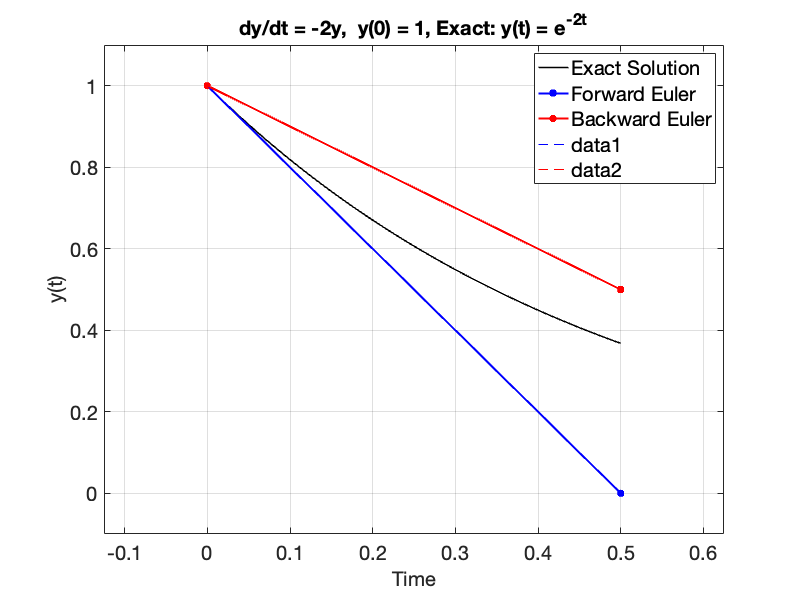
\includegraphics[width=1.2\textwidth]{figures/expVSimp.png}
         \end{figure}
      \column{0.5\textwidth}
         \centering
         Forward Euler (\textbf{explicit}):
         \begin{equation*}
            y_{n+1} = y_{n} + hy_{n}^{'}
         \end{equation*}
         \centering
         Backward Euler (\textbf{implicit}):
         \begin{equation*}
            y_{n+1} = y_{n} + hy_{n+1}^{'}
         \end{equation*}
   \end{columns}
\end{frame}

%%%%%%%%%%%%%%% EXERCISES
{%
   \setbeamertemplate{footline}{}
   \begin{frame}[standout]
	   Exercises
   \end{frame}
}

\begin{frame}{Exercises}
   \begin{itemize}
      \item[$\blacktriangleright$] Implement in MATLAB a function to perform the
         integration exploiting Euler forward and Backward method and test it on the ODE
         reported below then study the behaviour of the algorithms with respect to a
         multiplication factor k. (Analytical solution: $x = x_{0}exp(-t)$)
         \begin{equation*}
            \frac{dx}{dt} = -k * x
         \end{equation*}

      \item[$\blacktriangleright$] Solve the system of ODE reported below exploiting the
         builtin MATLAB function \color{blue} ode45 \color{black}.
         \begin{equation*}
            \begin{cases}
               \frac{dC_{A}}{dt} = -C_{A} \\
               \frac{dC_{B}}{dt} = C_{A} - C_{B} \\
               \frac{dC_{C}}{dt} = C_{B}
            \end{cases}
         \end{equation*}
   \end{itemize}
\end{frame}

\begin{frame}{}
   \begin{columns}[T]
      \column{0.3\textwidth}
      \begin{tikzpicture}[overlay, remember picture]
         \node[above right=1.7cm and .7cm of current page.south west]{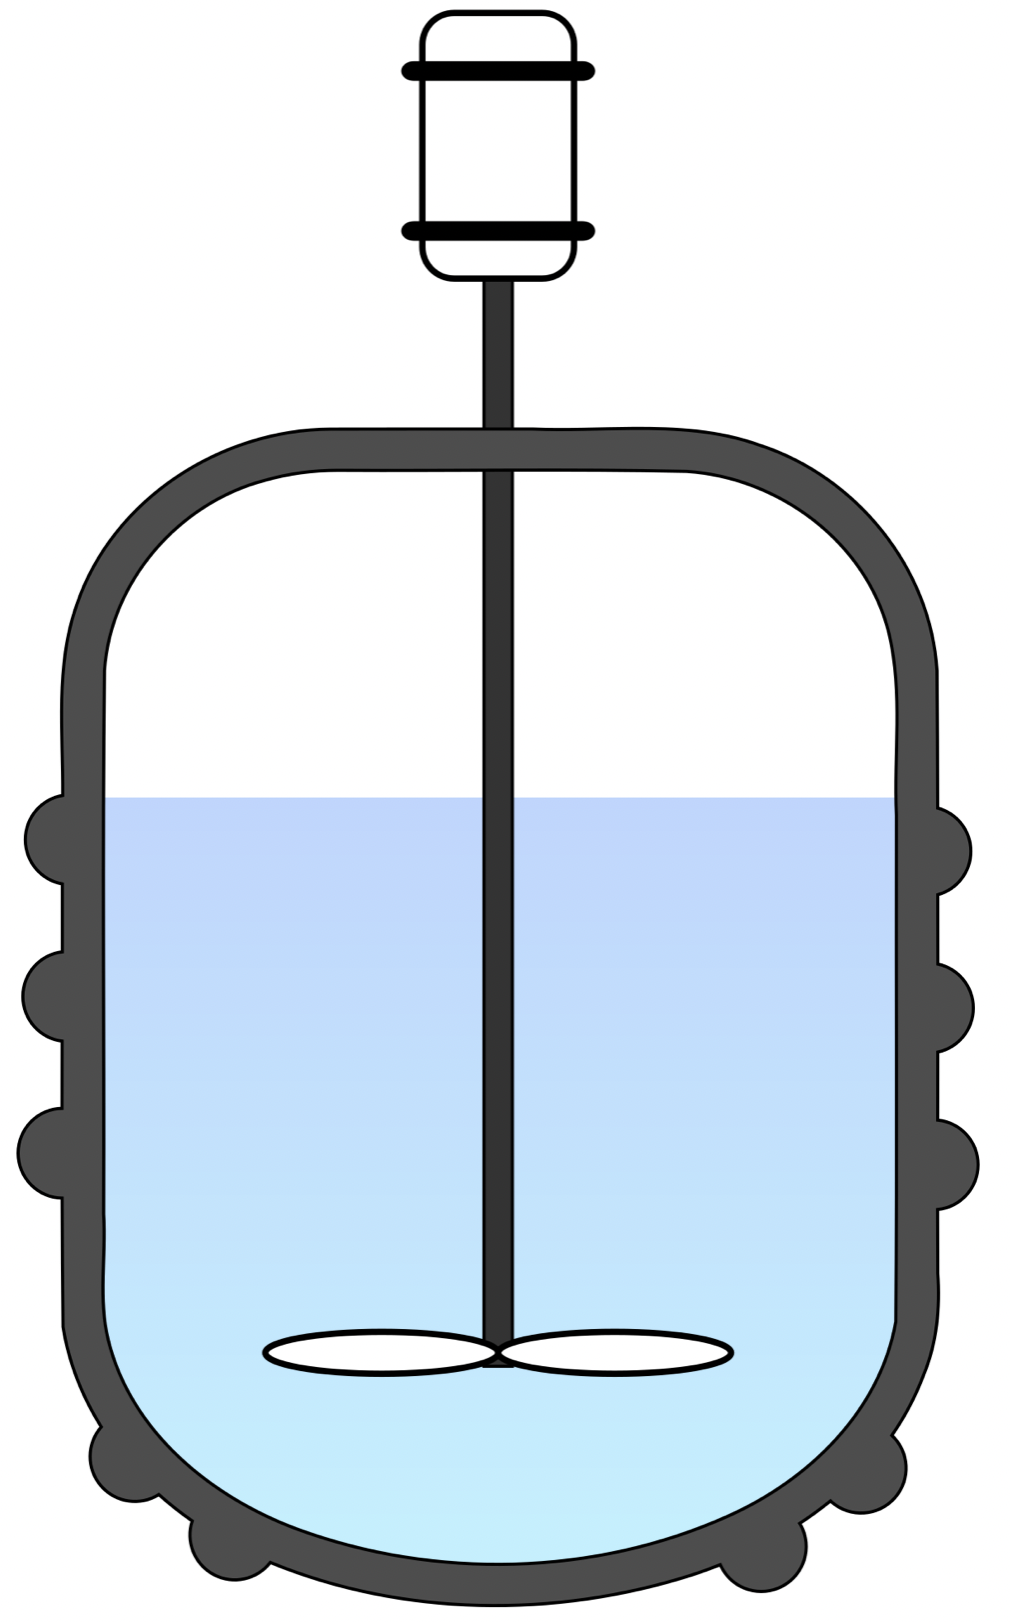
\includegraphics[width=3.5cm]{figures/batch.png}};
      \end{tikzpicture}
      \column{0.7\textwidth}
      \textbf{Design of isothermal batch reactor.} \\
      Compute the conversion (hereinafter denoted as $X_{A}$) of the reactant $A$
      occuring inside an isothermal batch reactor, in which takes place the following
      first order irreversible reaction:
      \begin{equation*}
         A \rightarrow B \: \: \: k = 0.01 \: \left[s^{-1}\right]
      \end{equation*}
   \end{columns}
\end{frame}

\begin{frame}{}
   Let's define the reaction rate ($r$) as:
   \begin{equation*}
      r = k \cdot C_{A}
   \end{equation*}

   Now write the rate of production/consumption of the two species taking part into the reaction:
   \begin{columns}[T]%beamer
      \column{5cm}
      \begin{equation*}
         \left\{
            \begin{aligned}
               R_{A} &= -k \cdot C_{A} \\
               R_{B} &= k \cdot C_{B}
            \end{aligned}
         \right .
      \end{equation*}
      \column{5cm}
      \begin{equation*}
         \left\{
            \begin{aligned}
               \frac{dC_{A}}{dt} &= -k \cdot C_{A} \\
               \frac{dC_{B}}{dt} &= k \cdot C_{A}
            \end{aligned}
            \right .
      \end{equation*}
   \end{columns}
\end{frame}

\begin{frame}{}
   Now let's focus on the first equation of the system:
   \begin{equation*}
      \frac{dC_{A}}{dt} = -k \cdot C_{A} \quad\text{given}\quad X_{A} = \frac{C_{A}^{0}-C_{A}}{C_{A}^{0}}
   \end{equation*}

   So the equation will become:

   \begin{equation*}
      -C_{A}^{0} \cdot \frac{dX}{dt} = -k\cdot C_{A}^{0}\cdot(1-X)
   \end{equation*}

   \begin{equation*}
      \frac{dX}{dt} = k \cdot (1 - X) \quad\text{with}\quad X(t = 0) = 0
   \end{equation*}
   \begin{equation*}
      \text{So the solution of the ordinary differential equation will be}\quad X(t) = 1 - exp(-k \cdot t)
   \end{equation*}
\end{frame}

\begin{frame}{}
   \begin{itemize}
      \item[$\blacktriangleright$] Solve the system of equations of Lotka-Volterra (x
         prey and y predator) and The Lorenz attractor to emulate a chaotic system:
         \begin{columns}[T]
         \column{0.5\textwidth}
            \centering
            Lotka-Volterra
            \begin{equation*}
               \begin{cases}
                  \frac{dx}{dt} = (\alpha - \beta y)x \\
                  \frac{dy}{dt} = (\gamma x - \delta)y
               \end{cases}
            \end{equation*}
            $\alpha = 0.3$, $\beta = 0.15$, $\gamma = 0.1$, $\delta = 0.1$.
         \column{0.5\textwidth}
            \centering
            Lorentz
            \begin{equation*}
               \begin{cases}
                  \frac{dx}{dt} = \sigma(y - x)\\
                  \frac{dy}{dt} = x(\rho - z) - y \\
                  \frac{dz}{dt} = xy - \beta z
               \end{cases}
            \end{equation*}
            $\beta = 8/3$, $\sigma = 10$, $\rho = 10$.
         \end{columns}
   \end{itemize}
\end{frame}


%%%%%%%%%%%%%%% CLOSING
{%
\setbeamertemplate{footline}{}
\begin{frame}[standout]
	Thank you for the attention!
\end{frame}
}

\end{document}
